\documentclass[12pt]{article}
%\documentclass[12pt,legalpaper]{article}
%\documentclass[14pt,legalpaper]{extarticle}
\usepackage{fullpage}
\usepackage{amsmath,amssymb}
\usepackage{mathptmx}
\usepackage{fancyhdr}
\usepackage{lastpage}
\usepackage{multicol}
\usepackage{graphicx}
\usepackage[aux]{rerunfilecheck}
\usepackage[rflt]{floatflt}

%\setlength{\textheight}{11.5in}

\reversemarginpar

\newcommand{\myimp}{\Rightarrow}
\newcommand{\myiff}{\Leftrightarrow}
\newcommand{\mynot}{\neg}
\newcommand{\myor}{\vee}
\newcommand{\myand}{\wedge}
\newcommand{\ds}{\displaystyle}

\DeclareSymbolFont{AMSb}{U}{msb}{m}{n}
\DeclareMathSymbol{\N}{\mathbin}{AMSb}{"4E}
\DeclareMathSymbol{\Z}{\mathbin}{AMSb}{"5A}
\DeclareMathSymbol{\R}{\mathbin}{AMSb}{"52}
\DeclareMathSymbol{\Q}{\mathbin}{AMSb}{"51}
\DeclareMathSymbol{\I}{\mathbin}{AMSb}{"49}
\DeclareMathSymbol{\C}{\mathbin}{AMSb}{"43}

\pagestyle{fancy}
\lhead{MATH 110 200930                                                     \\ 
  Sample Final Examination 2 \hspace{0.75in} Page\ \thepage\ of \pageref{LastPage}  \\ 
  Time: 3 hours                                                            \\
  \quad                                                                      }
%\chead{\quad                                                              \\ 
%       Page\ \thepage\ of \pageref{LastPage}                              \\ 
%	\quad                                                                }
\chead{}
\rhead{Name: \underline{\hspace{2in}}        \\ 
       Student \#: \underline{\hspace{2in}}  \\ 
       Section: \underline{\hspace{2in}}     \\
       \quad                                   }
\cfoot{}
\addtolength{\headheight}{\baselineskip}
\addtolength{\headheight}{\baselineskip}
\addtolength{\headheight}{\baselineskip}
\addtolength{\headheight}{\baselineskip}
\renewcommand{\headrulewidth}{0pt}
\fancypagestyle{plain}{%
  \lhead{}
  \chead{FIRST NATIONS UNIVERSITY OF CANADA                \\
    DEPARTMENT OF SCIENCE \\
    MATH 110 200930 \\
  }
  \rhead{}
  \cfoot{Page\ \thepage\ of \pageref{LastPage}}
}

\title{Sample Final Examination 2}
\author{Edward Doolittle, Martin Argerami, Sergei Panafidin, Richard McIntosh, Fotini Labropulu, L.\ Dame}

\begin{document}
\thispagestyle{plain}
%\maketitle

\begin{center}
  \LARGE{MATH 110 200930 Sample Final Examination 2}
\end{center}

\begin{flushleft}
\quad\\
Time:  3 hours                  \hfill       Name: \underline{\hspace{2in}}  \\
Instructors:                    \hfill Student \#: \underline{\hspace{2in}}  \\
\quad Dr. Edward Doolittle      \hfill    Section: \underline{\hspace{2in}}  \\
\end{flushleft}


\noindent
You have 3 hours to do each of the following questions.
The test is worth a total of 100 marks.
Please\marginpar{\footnotesize{(marks)}} justify your conclusions and
show all your work.
A non-programmable calculator of the type mentioned in the course outline
is permitted; no other aids are permitted.
%Use the backs of the pages for rough work.

\begin{enumerate}
\item Find\marginpar{\footnotesize{(12)}}
  $\ds \frac{dy}{dx}$ in each of the following cases.  (You do not have
  to simplify your answers.)
  \begin{enumerate}
  \item $\ds y = \frac{1}{x^{3/2}} - x^{2/3} + \sin x$
\vfill
  \item $\ds y = \frac{\cos(x^2)}{\cos^2(x)}$
\vfill
  \item $\ds \sqrt{x+y+1} = 1 + x^2y^2$
\vfill
  \item $\ds y = \int_1^x \sqrt{\frac{t^2+1}{t^4+1}} \; dt$
\vfill
  \end{enumerate}
\newpage
\item Evaluate\marginpar{\footnotesize{(12)}}
  the following limits if they exist.
  \begin{enumerate}
  \item $\ds \lim_{x\to 0} \frac{\sin \pi x}{x}$
\vfill
  \item $\ds \lim_{x\to \infty} \frac{2x^3-7}{(1-x^2)(4x+7)}$
\vfill
  \item $\ds \lim_{x\to -4} \frac{x^2+5x+4}{x^2+3x-4}$
\vfill
  \item $\ds \lim_{h\to 7} \frac{\sqrt{h+2}-3}{h-7}$
\vfill
  \end{enumerate}
\newpage
  \begin{center}
    \includegraphics[width=6in]{grph.eps}
  \end{center}
\item Consider\marginpar{\footnotesize{(6)}} 
  the above graph of the function $f$.
  \begin{enumerate}
  \item List all $x$ for which $f$ fails to be continuous.
\vfill
  \item List all $x$ for which $f$ fails to be differentiable.
\vfill
  \end{enumerate}
\newpage
\item Use\marginpar{\footnotesize{(6)}} 
  the Intermediate Value Theorem to show that $f(x)=x^4+x-3$ must have
  at least one root in the interval $[1,2]$.
\vfill
\item Find\marginpar{\footnotesize{(10)}}
  the equation of the tangent line to the curve $\ds x^2+\frac{1}{xy}-1=y^2$
  at the point $(1,1)$.
\vfill
\vfill
\newpage
\item A\marginpar{\footnotesize{(10)}} 
  spherical hot air balloon is inflated at the rate of $0.3$ m$^3$/s.  At
  what rate is the radius $r$ of the balloon increasing when $r=2$ m?
  (The volume of a sphere of radius $r$ is $(4/3)\pi r^3$.)
\vfill
\newpage
\item Let\marginpar{\footnotesize{(10)}}
  $f(x)=x^3+3x^2-9x-2$.
  \begin{enumerate}
  \item Identify all (if any) \\
    local maxima \hrulefill \\
    local minima \hrulefill \\
    points of inflection \hrulefill \\
    asymptotes \hrulefill 
  \item Determine the intervals on which $f$ is \\
    increasing \hrulefill \\
    decreasing \hrulefill \\
    concave up \hrulefill \\
    concave down \hrulefill
  \end{enumerate}
  Use the space below to show your work for parts (a) and (b).  If more
  space is required, use the back of the facing page and indicate that
  you have done so.
\vfill
\newpage
\addtocounter{enumi}{-1}
\item (continued)
  \begin{enumerate}
  \setcounter{enumii}{2}
  \item Use the information in parts (a) and (b) to sketch a graph of $f$.  
\vfill
  \end{enumerate}
\newpage
\item A\marginpar{\footnotesize{(10)}} 
  flower garden of total area $12$ m$^2$ is to be constructed in front of 
  a house.  The garden has to be fenced on three sides.  The price of the 
  fence used on the two opposite sides is \$3 per meter, and on the third
  side \$2 per meter.  Find the dimensions of the garden that would minimize
  the cost of the fence.
\vfill
\newpage
\item Find\marginpar{\footnotesize{(10)}} 
  the area of the region bounded by the curves $y=x^2-2x$ and $y=x$.
\vfill
\newpage
\item Evaluate\marginpar{\footnotesize{(12)}}
  the following integrals.
  \begin{enumerate}
  \item $\ds \int x \; \sin(1+x^2) \; dx$
\vfill
  \item $\ds \int \left(\frac{1}{x} + \sqrt{x}\right)^2 \; dx$
\vfill
  \item $\ds \int_1^2 \frac{1}{x^2} \cos\left(\frac{\pi}{x}\right) \; dx$
\vfill
  \item $\ds \int_0^3 \sqrt{3x+16} \; dx$
\vfill
  \end{enumerate}
\end{enumerate}
\end{document}

